\documentclass[conference,a4paper]{IEEEtran}
% Shared IEEE-compatible packages. Compiles with pdfLaTeX on Overleaf.
\usepackage[T1]{fontenc}
\usepackage[utf8]{inputenc}
\usepackage{cite}
\usepackage{amsmath,amssymb}
\usepackage{graphicx}
\usepackage{booktabs,array,tabularx}
\usepackage{url}
\usepackage{xcolor}
\usepackage{tikz}
\usepackage{placeins}
\usetikzlibrary{arrows.meta,positioning,shapes.geometric,fit}
\usepackage[breaklinks=true,hidelinks]{hyperref}
\hypersetup{pdfauthor={},pdfsubject={FinPilot AI synthetic sandbox competition documentation}}
\graphicspath{{figures/}}
\newcommand{\project}{FinPilot AI}
\newcommand{\RepoLink}{\url{https://github.com/Shariar-Joy/finpilot-ai}}
\newcommand{\VerifiedCI}{\href{https://github.com/Shariar-Joy/finpilot-ai/actions/runs/39220992552}{verified CI run 39220992552}}
\newcommand{\field}[1]{\rule{#1}{0.35pt}}
\newcommand{\teamAuthors}{\author{%
\IEEEauthorblockN{\field{48mm}}
\IEEEauthorblockA{Team member 1\\Institution: \field{34mm}\\Email: \field{40mm}}
\and
\IEEEauthorblockN{\field{48mm}}
\IEEEauthorblockA{Team member 2\\Institution: \field{34mm}\\Email: \field{40mm}}}}
\newcolumntype{L}[1]{>{\raggedright\arraybackslash}p{#1}}
\definecolor{navy}{HTML}{16233B}
\definecolor{teal}{HTML}{177F78}
\definecolor{lightgray}{HTML}{F2F4F7}
\tikzset{box/.style={draw=navy,rounded corners=2pt,fill=lightgray,align=center,font=\footnotesize,minimum height=11mm,text width=28mm},flow/.style={-{Stealth[length=2mm]},thick,draw=navy},optional/.style={flow,dashed,draw=teal}}
% Generated from actual executed results. Do not change counts by hand.
\newcommand{\UnitTests}{61}
\newcommand{\BrowserTests}{4}
\newcommand{\PythonTests}{8}
\newcommand{\RecordedTransactions}{134}
\newcommand{\AgentMedian}{0.534}
\newcommand{\AgentPninetyfive}{0.827}
\newcommand{\EvidenceDate}{19 October 2026}
\newcommand{\DemoSeconds}{84}


\title{FinPilot AI: A Personal Finance Agent with Deterministic Tools and Explicit Approval}
\teamAuthors
\begin{document}
\maketitle
\begin{abstract}
Personal finance assistants need to turn questions into useful actions while retaining numerical accuracy and user control. This paper presents FinPilot AI, a working synthetic-account sandbox for budgeting, transaction analysis, recurring bills, and explainable spending insights. The system separates optional language-model tool planning from deterministic financial calculations and authorization. Read tools return ledger-derived evidence; proposal tools prepare exact changes; mutation tools require an expiring, single-use token bound to the user and canonical payload. Budget changes, approval consumption, and audit records commit atomically. A keyless deterministic agent completes the same demonstration without an external model. On a fixed 90-day dataset containing \RecordedTransactions{} synthetic transactions, the principal scenario explains a dining-spending increase and proposes a next-month budget of USD~518.48 from USD~648.10 of recorded spending. Verification comprises \UnitTests{} TypeScript domain/API tests, \BrowserTests{} Chromium scenarios, and \PythonTests{} FastAPI tests. These checks establish bounded functional and security invariants; they do not establish financial-advice quality, production scalability, or regulatory compliance. Source, execution evidence, and reproducible setup accompany the implementation.
\end{abstract}
\begin{IEEEkeywords}
personal finance, financial agents, deterministic tools, explicit approval, explainability, sandbox evaluation
\end{IEEEkeywords}

\section{Introduction}
An assistant that describes spending without completing an approved financial task provides limited operational value. Conversely, granting a language model unrestricted write access creates a permission boundary that is difficult for a user to inspect. Personal finance therefore requires a workflow that connects explanation, review, execution, and evidence.

FinPilot AI addresses Topic A, Personal Finance Assistant, in the 2026 Shenzhen International FinTech Competition. The supplied appendix asks for actionable budgeting, bill analysis, and spending insights, and weights task completion at 40\%, security and compliance at 30\%, and innovation and interaction at 30\%~\cite{competition}. Our implementation operates exclusively on synthetic sandbox records. It performs no bank connection, payment, securities transaction, or external notification delivery.

The engineering contributions are: (1) a working tool-based finance workflow with a deterministic fallback; (2) an explicit authorization protocol that binds approval to the exact reviewed payload; and (3) a reproducible evaluation package linking calculations, browser actions, and sanitized execution records. These contributions describe an implemented system; we do not claim a new financial forecasting algorithm or a benchmark advantage over existing assistants.

\section{Related Work and Design Position}
ReAct studies language-model reasoning interleaved with environment actions~\cite{react}. FinPilot adopts the practical idea that an assistant should invoke inspectable tools, but its optional provider uses a bounded planning request rather than an unrestricted iterative reasoning loop. The planner selects operations; application code supplies numeric results and the final grounded response.

OWASP identifies excessive permissions and autonomy as sources of harmful agent actions~\cite{owaspagency}. The design responds by exposing only narrow read/proposal functions to the model and placing the write decision behind explicit user review. NIST AI RMF offers broader risk-management guidance~\cite{nist}; it informs the separation of implemented controls, measured behavior, and residual risks rather than serving as a certification claim. The provider integration uses the Responses function-calling interface~\cite{openai}. The paper follows IEEE conference layout conventions~\cite{ieeetemplate}; it is competition documentation, not an IEEE publication or endorsement.

\section{Requirements and System Scope}
The intended user can inspect synthetic income and expenses, upload a validated CSV, identify recurring payments, create category budgets, and ask the agent to propose a change. The principal task is: explain why dining spending increased this month and set the next month's dining budget 20\% below recorded current-month dining spending. A successful run must present evidence and an exact proposal, apply only after approval, and leave finances unchanged after rejection.

Three invariants guide the implementation. First, financial amounts are signed integer minor units, with no floating-point values stored as money. Second, every protected read/write derives ownership from a verified session rather than a user-selected identifier. Third, a model response cannot authorize a financial mutation. Direct UI forms require explicit confirmation; agent-originated mutations additionally require the proposal token.

\begin{figure*}[t]
\centering
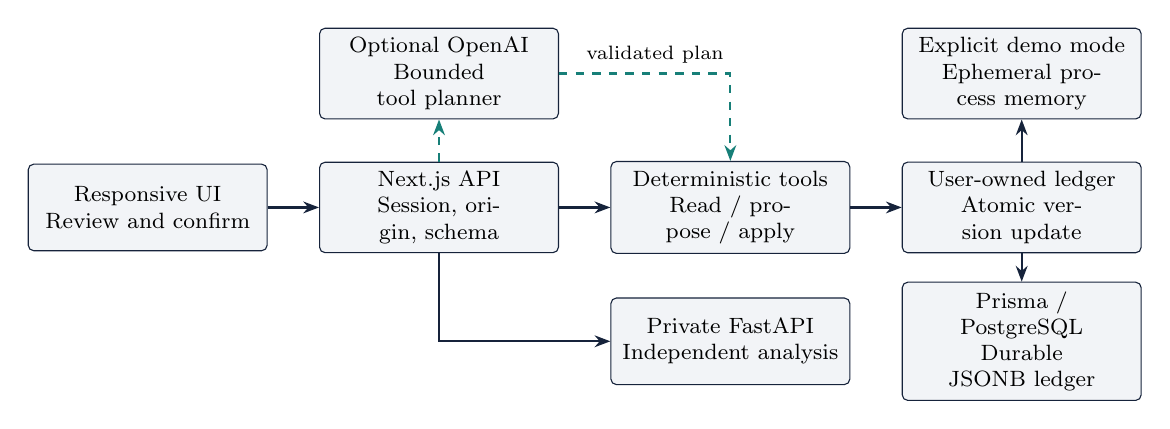
\begin{tikzpicture}[x=1cm,y=1cm]
\node[box] (ui) at (0,0) {Responsive UI\\Review and confirm};
\node[box] (api) at (3.7,0) {Next.js API\\Session, origin, schema};
\node[box] (tools) at (7.4,0) {Deterministic tools\\Read / propose / apply};
\node[box] (repo) at (11.1,0) {User-owned ledger\\Atomic version update};
\node[box] (llm) at (3.7,1.7) {Optional OpenAI\\Bounded tool planner};
\node[box] (python) at (7.4,-1.7) {Private FastAPI\\Independent analysis};
\node[box] (pg) at (11.1,-1.7) {Prisma / PostgreSQL\\Durable JSONB ledger};
\node[box] (mem) at (11.1,1.7) {Explicit demo mode\\Ephemeral process memory};
\draw[flow] (ui)--(api);
\draw[flow] (api)--(tools);
\draw[flow] (tools)--(repo);
\draw[optional] (api)--(llm);
\draw[optional] (llm)-| node[pos=.28,above,font=\scriptsize]{validated plan} (tools);
\draw[flow] (api.south) |- (python.west);
\draw[flow] (repo)--(pg);
\draw[flow] (repo)--(mem);
\end{tikzpicture}

\caption{Implemented architecture. Solid arrows show application/service boundaries; dashed arrows denote optional provider planning. Repository selection is explicit: PostgreSQL persistence or a visibly ephemeral single-process demo. No component connects to a real bank or payment rail.}
\label{fig:architecture}
\end{figure*}

\section{System Architecture}
\subsection{Application and Analysis Boundaries}
The interface uses Next.js App Router, strict TypeScript, Tailwind CSS, a shared responsive design system, and Recharts. Routes cover the landing page, authentication, dashboard, transactions, budgets, bills, insights, agent, audit activity, and settings. The same-origin API validates requests with Zod. Merchant names and uploaded text remain untrusted data and are rendered as escaped text.

Deterministic TypeScript functions implement totals, comparisons, recurrence, anomalies, and budget calculations. A private, stateless Python FastAPI service independently recomputes monthly financial totals from authenticated user-scoped records. The application sends only transaction identifiers, dates, categories, and integer amounts. A shared service token and a three-second timeout protect this optional boundary; Python has no mutation or database authority.

\subsection{Persistence and Atomicity}
Prisma models relational users, revocable sessions, and a per-user ledger aggregate. The PostgreSQL ledger stores financial arrays, approvals, conversation records, and audit events in JSONB. A mutation reads the user's version, copies the aggregate, applies a synchronous operation, and executes an update conditioned on that version. A conflicting update retries up to five times. Consequently, approval consumption, budget/reminder change, and audit append share one committed update. The memory repository uses a mutex and the same copy-before-mutate semantics.

The aggregate deliberately favors reviewable atomicity over analytical scale. Rewriting a whole JSONB document is unsuitable for very large ledgers; normalized transaction tables and an independently protected audit store are future work. When no database is configured, the application visibly identifies ephemeral memory mode. Restarting that process loses data and sessions; a configured database failure never silently falls back.

\subsection{Sessions and API Controls}
Registered passwords use bcrypt with cost 12 and a 72-byte UTF-8 bound. An encrypted HttpOnly, SameSite cookie contains a random session token and user identity; the server stores only the token hash with an eight-hour expiry. Logout revokes the server record. HTTPS configuration adds the Secure cookie flag. Write requests require the expected Origin and JSON content type. Rate limits, string/amount bounds, and incremental request-body limits protect the HTTP boundary. Process-local limits require a shared gateway for multi-instance deployment.

\section{Deterministic Financial Methods}
\subsection{Integer Arithmetic and Monthly Summaries}
Let $a_i\in\mathbb{Z}$ be signed transaction cents for month $m$. Income, expenses, and net savings are
\begin{equation}
I_m=\sum_{i:a_i>0}a_i,\quad E_m=-\sum_{i:a_i<0}a_i,\quad S_m=I_m-E_m.
\end{equation}
Amount sign determines cash direction; categories are labels. CSV decimals are assembled from whole/fraction digits, not multiplied from binary floating-point input. Every operand and aggregate must remain a safe integer. Calendar accounting uses UTC.

For spending $E_{m,c}$ in category $c$ and a whole-number percentage reduction $r$, the proposed cent limit is
\begin{equation}
B_{m+1,c}=\left\lfloor\frac{E_{m,c}(100-r)+50}{100}\right\rfloor .
\label{eq:budget}
\end{equation}
The numerator is evaluated with BigInt, yielding round-half-up rounding to cents. Limits must be positive and within the supported amount bound. The agent does not infer a percentage when the user has omitted one or entered an unsupported fractional reduction.

\subsection{Comparisons and Source Evidence}
The current month's spending is compared through today's UTC day with the same days of the previous month. The result contains totals, purchase counts, average purchase size, and largest purchases with transaction IDs. Historical requested months compare full recorded months. Descriptions report observed differences without inferring unobserved motives. A budget proposal uses all currently recorded spending in the source month; later purchases do not silently alter the payload already reviewed by the user.

\subsection{Recurring Bills and Unusual Purchases}
Recurring-payment inference groups expenses by normalized merchant, requires at least three observations, and checks each consecutive interval is 25--35 days. Every amount must be within 15\% of the upper median. The next estimated date advances by calendar month, clamping month-end dates. The output includes supporting transaction IDs; it is an inferred pattern, not a contractual schedule.

An unusual-purchase flag requires at least five strictly earlier category expenses. With prior upper median $M_c$, expense $x$ is flagged when
\begin{equation}
x>\max(3M_c,10000)
\end{equation}
in cents. Same-day purchases are excluded from the baseline. These transparent rules produce descriptive flags rather than fraud determinations. No real-world detection precision or recall is claimed.

\subsection{Atomic CSV Import}
Imports accept at most 512~KB and 2,000 rows with ordered date, merchant, amount, and category headers. Calendar dates, merchant bounds, category membership, decimal precision, and amounts are validated for the entire batch before a write. A fingerprint of date, normalized merchant, and signed amount identifies duplicates both within a batch and against existing records. Validation reruns inside the atomic mutation. This deliberately treats identical same-day purchases as duplicates, a documented limitation. Exported formula-prefixed merchant cells receive an apostrophe before CSV quoting.

\begin{figure*}[t]
\centering
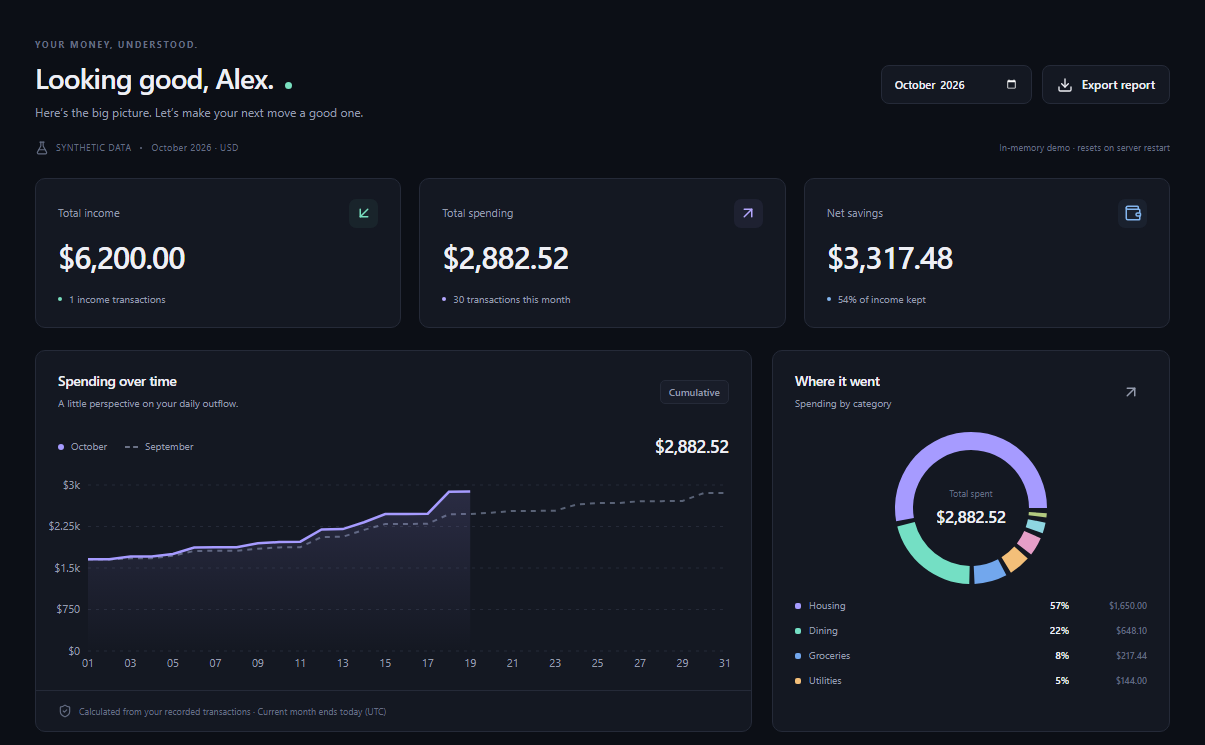
\includegraphics[width=\textwidth]{dashboard.png}
\caption{Actual FinPilot dashboard captured from the running application with synthetic data. Cards and charts are computed from the ledger; screenshots are interface evidence, not generated mockups. The fixed-seed numeric experiment is reported separately in Table~\ref{tab:golden}.}
\label{fig:dashboard}
\end{figure*}

\section{Tool Orchestration and Approval}
\subsection{Permission Tiers}
The read tier comprises spending summaries, transaction listing, month comparison, budget status, recurring bills, and anomaly explanations. The proposal tier prepares budget changes and named bill reminders. The mutation tier comprises \texttt{apply\_budget\_change} and \texttt{apply\_bill\_reminder}; these operations are not exposed to the model. A keyless parser supports the demonstrated finance intents using the same real tool executor. Optional provider planning uses strict function schemas, an eight-call cap, a 12-second provider timeout, and a 20-second execution guard. Provider failures or malformed plans choose the fallback; valid but unsupported requests return a bounded error or clarification rather than inventing an action.

\begin{figure}[t]
\centering
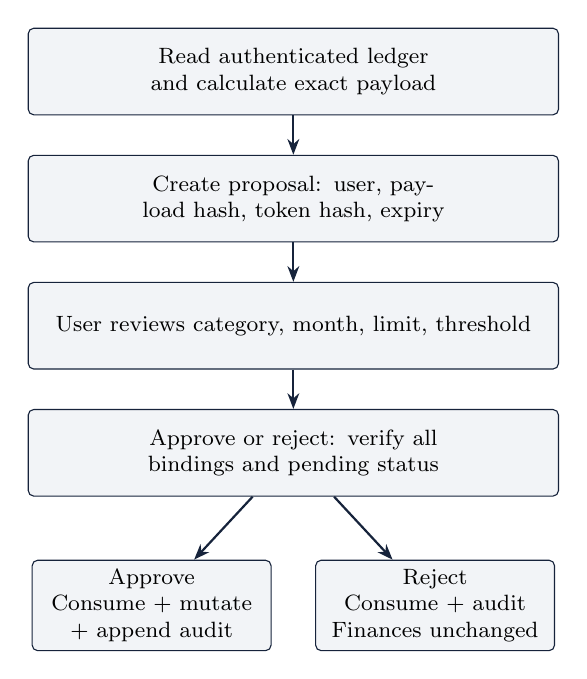
\begin{tikzpicture}[node distance=5mm]
\node[box,text width=65mm] (read) {Read authenticated ledger and calculate exact payload};
\node[box,text width=65mm,below=of read] (propose) {Create proposal: user, payload hash, token hash, expiry};
\node[box,text width=65mm,below=of propose] (review) {User reviews category, month, limit, threshold};
\node[box,text width=65mm,below=of review] (verify) {Approve or reject: verify all bindings and pending status};
\node[box,text width=28mm,below=8mm of verify,xshift=-18mm] (apply) {Approve\\Consume + mutate\\+ append audit};
\node[box,text width=28mm,below=8mm of verify,xshift=18mm] (reject) {Reject\\Consume + audit\\Finances unchanged};
\draw[flow] (read)--(propose);
\draw[flow] (propose)--(review);
\draw[flow] (review)--(verify);
\draw[flow] (verify)--(apply);
\draw[flow] (verify)--(reject);
\end{tikzpicture}

\caption{Approval and rejection share an exact-payload verification step. A failed binding check cannot reach either decision commit; successful decisions consume the token exactly once.}
\label{fig:approval}
\end{figure}

\subsection{Exact-Payload Approval Protocol}
A proposal contains user identity $u$, canonical payload hash $h_p$, token hash $h_t$, expiry $e$, and status. The client receives a cryptographically random 256-bit token once. Application state stores only its hash. Approval or rejection is accepted only when
\begin{align}
u_{session}&=u_{proposal},\\
H(\operatorname{canon}(p_{request}))&=h_p,\\
H(t_{request})&=h_t,\\
\operatorname{status}&=\operatorname{pending},\\
\operatorname{now}&<e.
\end{align}
Canonical JSON sorts object keys. Token hashes are compared with a timing-safe function. Expiry is five minutes. A successful approval changes the budget/reminder, consumes the token, updates the visible timeline, and appends an audit event. Rejection consumes the token and records the decision while leaving financial arrays unchanged. Replay, cross-user, modified-payload, and expired requests fail. Optimistic version checks prevent two concurrent requests from applying the same token twice.

\section{Evaluation}
\subsection{Reproducible Setup}
The fixed seed date is 19 October 2026 at 12:00 UTC. Ninety calendar days produce \RecordedTransactions{} synthetic transactions across income, housing, dining, groceries, transport, utilities, shopping, and subscriptions. Node.js 24.13.0 and Python 3.14.2 were used on Windows. The deployed-framework build uses Next.js 16.4.2 and Prisma 6.19.3. Evaluation code and exact logs are supplied in the repository~\cite{repo}. No paid model call, human-subject study, real bank account, or production financial dataset is included.

\begin{table}[t]
\caption{Observed synthetic golden-scenario values}
\label{tab:golden}
\centering\small
\begin{tabular}{L{51mm}r}
\toprule Measurement & Recorded value\\\midrule
Dining, October 1--19 & USD 648.10\\
Dining, September 1--19 & USD 241.50\\
Purchase count, each period & 17\\
Mean purchase, October / September & USD 38.12 / 14.21\\
Largest October dining purchase & USD 248.00\\
Proposed November limit, 20\% lower & USD 518.48\\
\bottomrule
\end{tabular}
\end{table}

\subsection{Task Completion}
Table~\ref{tab:golden} reports the actual tool results. Spending rose because the recorded purchase sizes increased; the count remained equal. The largest current-period transaction is linked by its generated source identifier. Equation~\eqref{eq:budget} maps 64,810 cents to 51,848 cents. The browser scenario first rejects the proposal and compares budgets before/after, then runs a new proposal, approves it, checks the exact target budget, and observes both decisions in the audit log. A rejected decision is therefore demonstrated as an unchanged financial state rather than merely a conversational acknowledgement.

\subsection{Verification Results and Performance Scope}
\begin{table}[t]
\caption{Executed verification and its scope}
\centering\small
\begin{tabular}{L{43mm}L{36mm}}
\toprule Check & Observed outcome\\\midrule
TypeScript domain/API suite & \UnitTests{} passed\\
Chromium end-to-end scenarios & \BrowserTests{} passed\\
FastAPI validation/unit suite & \PythonTests{} passed\\
Lint, strict types, seed, build & Passed; exact logs provided\\
Production Next.js/FastAPI link & Exact totals; missing token: 401\\
Live paid-provider execution & Not exercised\\
Local PostgreSQL connection & Not exercised locally\\
Remote PostgreSQL 17 & Migration + 61 checks passed\\
\bottomrule
\end{tabular}
\label{tab:verification}
\end{table}

The tests cover integer conversion, total precision, CSV rollback/deduplication, recurrence, anomaly rules, cross-user access, session revocation, approval binding, concurrency, and browser workflows. Review regression cases additionally prevent an unknown merchant from being replaced by another bill, a missing/fractional percentage from becoming a guessed budget, and a historical summary from being described using current-month totals. Provider responses are mocked to exercise the boundary without spending or transmitting credentials.

A separate deterministic microbenchmark performs ten warm-up and 100 measured runs on newly seeded copies. Median execution is \AgentMedian{}~ms and the 95th percentile is \AgentPninetyfive{}~ms on the local machine. Timing excludes seed construction, HTTP, rendering, database access, and all model latency. It is a narrow engineering measurement, not an end-to-end service-level guarantee or comparative performance claim. Machine-readable results and the exact script accompany the source.

\section{Limitations and Deployment Conditions}
Verification checks specific invariants, not arbitrary-language correctness or the absence of all vulnerabilities. The fallback supports bounded finance intents rather than general conversation. Optional model-selected proposals may still be semantically wrong; the user reviews the exact change. No model benchmark, user acceptance study, financial-advice outcome evaluation, or statistical anomaly-quality experiment was conducted.

The local environment lacked a running Docker/PostgreSQL service. Remote Ubuntu CI subsequently applied the migration to PostgreSQL 17 and passed the same 61 domain/API cases, including repository concurrency and rollback; the application job also passed build, Python, and browser checks (\VerifiedCI). Repeated adapter runs are not additional unique tests. This does not verify target deployment or restart recovery. The JSONB aggregate, process-local rate limits, inline-script CSP allowance, session cleanup, and absence of MFA/recovery require further work before use with real customers. A trusted TLS gateway and persistent secrets are deployment requirements. No certification, regulated financial advice, or payment capability is asserted.

\section{Conclusion}
FinPilot demonstrates a complete sandbox task: an expense question leads to source-backed analysis, a deterministic proposal, an explicit decision, and an auditable state transition. The principal result is the implemented separation of language planning, financial computation, and mutation authority. The supplied code, tests, screenshots, and logs make that result inspectable. Further evaluation should prioritize durable deployment verification, broader intent coverage, independent security assessment, and user studies before any real-finance use.

\section*{Reproducibility and Authorship}
Source and setup: \RepoLink. All evaluation records are synthetic. Team identity, affiliations, and contributions must be completed by the two members. Implementation and documentation were prepared with AI-assisted engineering; the team must review all claims, dependencies, and the organizer's applicable independence/IP rules before making any authorship declaration. No signatures, affiliations, funding, or external endorsements are supplied by this document.

\FloatBarrier
\bibliographystyle{IEEEtran}
\bibliography{references}
\end{document}
